\subsection{Behaviour of Model under Parameter Changes}
\label{sec:og.param.effects}

To replicate the dynamics seen in the model, it is helpful to know, how the model changes along the areas of the same period.
\Cref{fig:yunus.function.evolution} shows, how the model function changes along the area of period 12.
In the figure, there are three functions in three different colors.
The first function is blue and it is the model with parameters $E_0 = 15.9, \chi_0 = 0.11$.
The second function is purple and it is the model at the point $E_0 = 17.45, \chi_0 = 0.2$.
The last function is red and it is the model with parameters $E_0 = 19, \chi_0 = 0.29$.

\begin{figure}
    \centering
    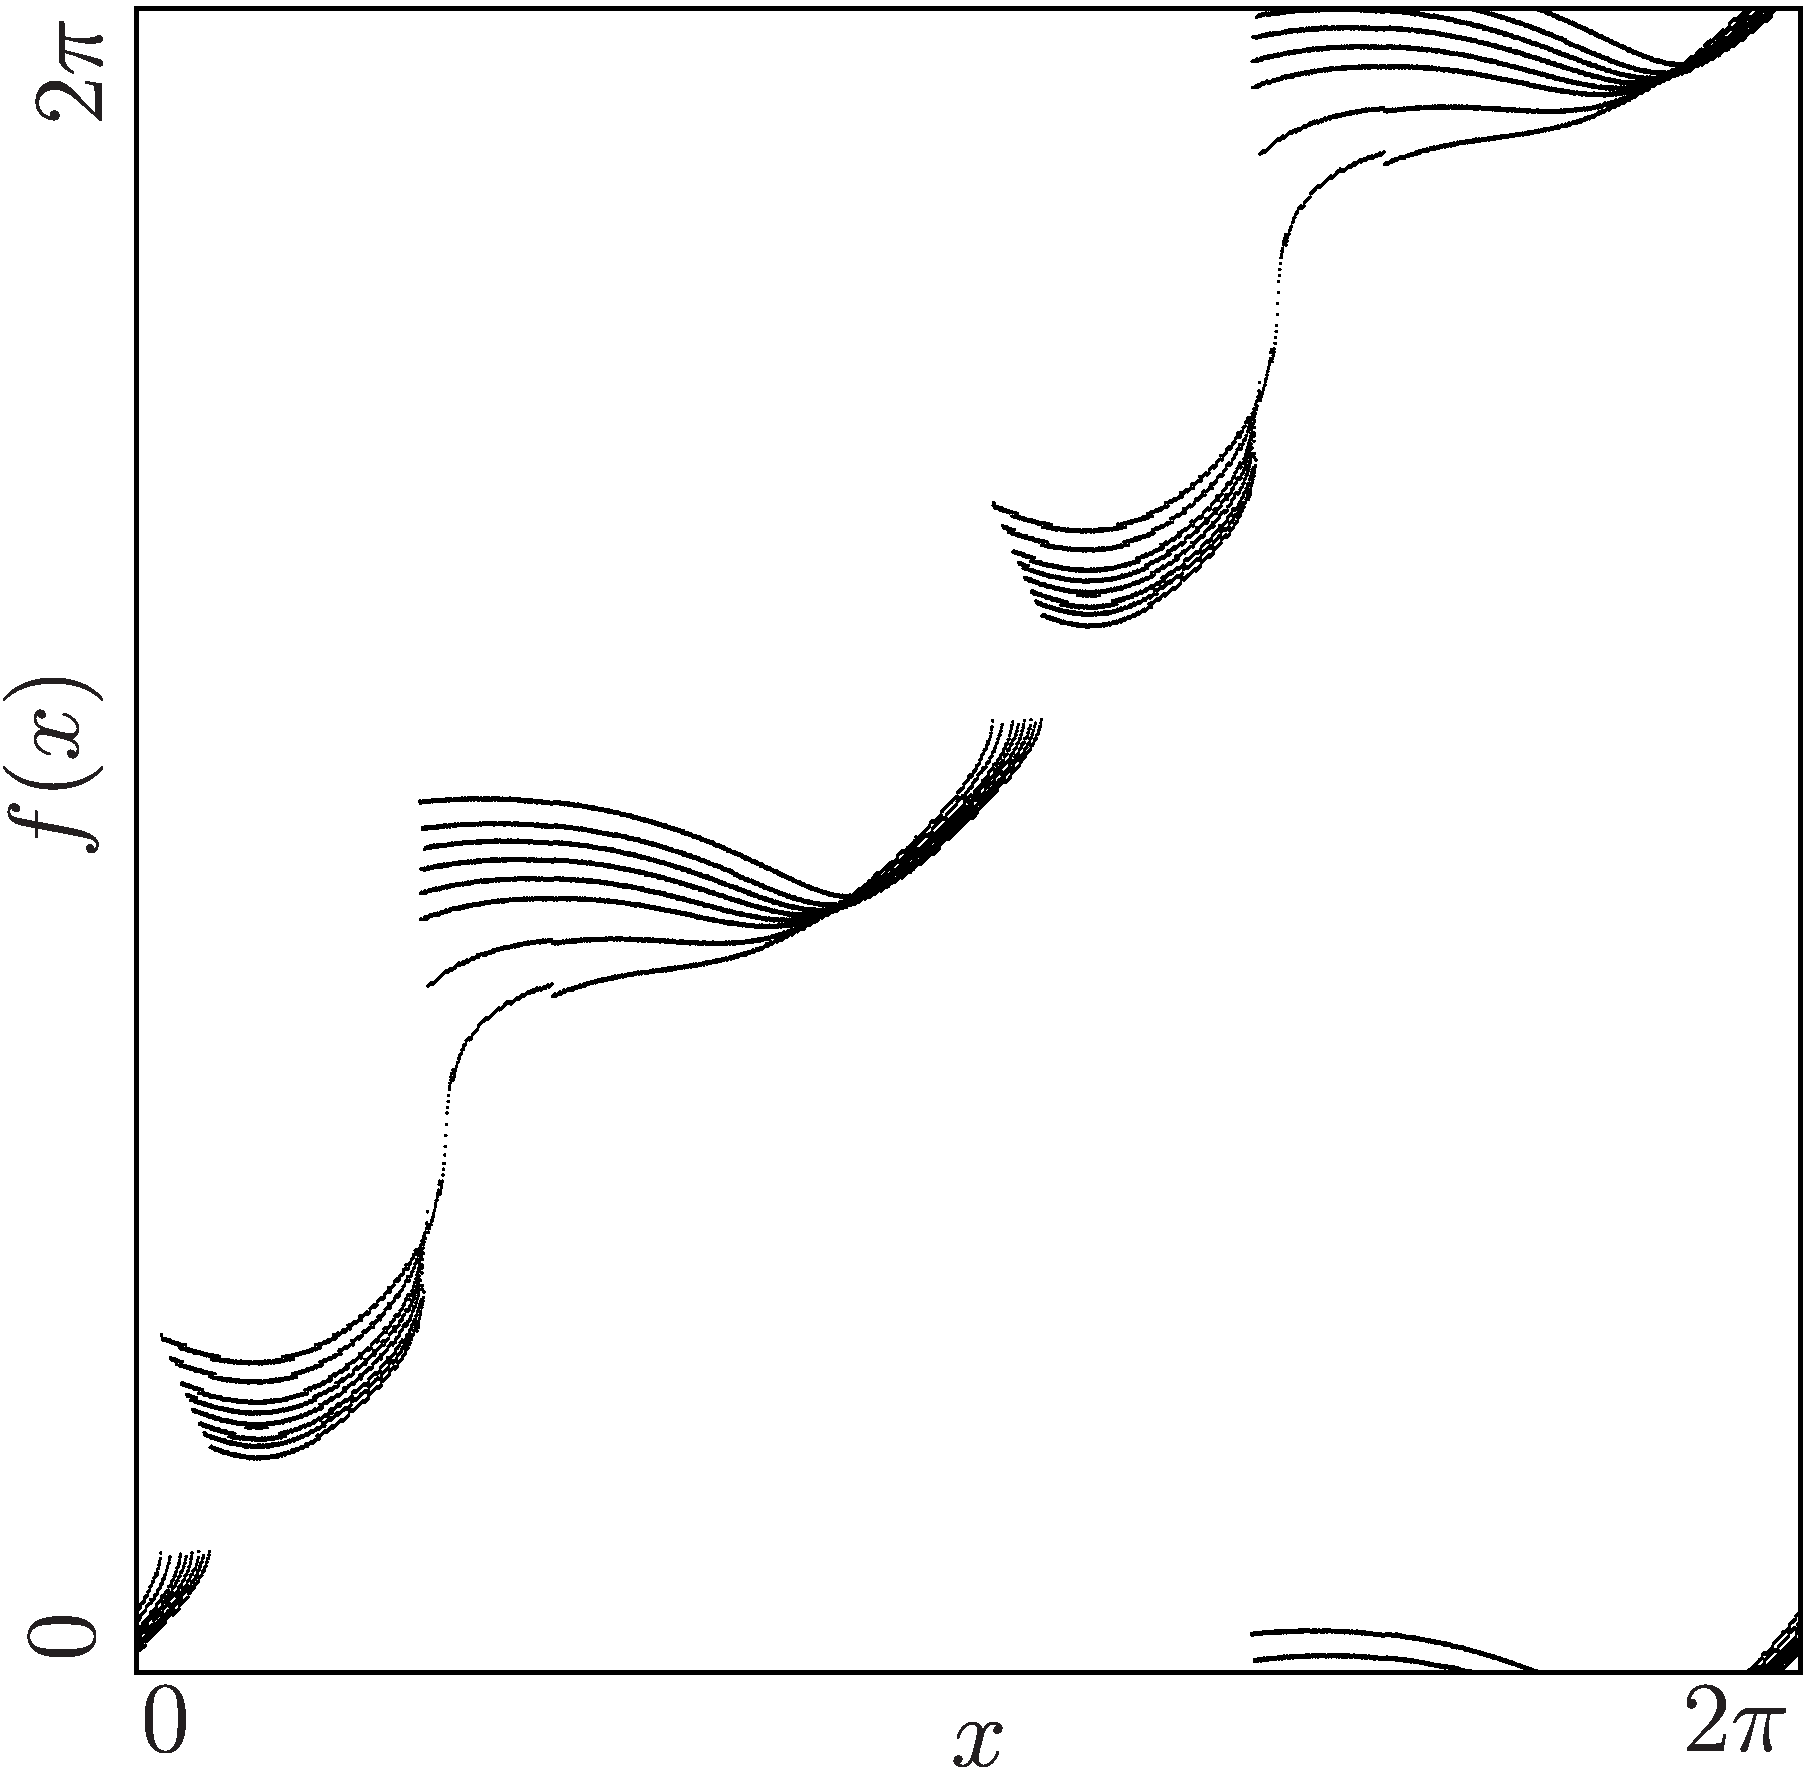
\includegraphics[width=0.6\textwidth]{99_Yunus/ParameterEffects/E0_hi_P12/illustration.png}
    \caption{Evolution of the Original Model Function}
    \label{fig:yunus.function.evolution}
\end{figure}

The most notable changes are
\begin{enumerate*}
    \item Branches $\A$ and $\C$ move upwards while the left part moves upwards more
    \item The left part of branches $\B$ and $\D$ move downwards 
    \item The local minima of these branches move to the left and downwards.
\end{enumerate*}
Smaller changes include
\begin{enumerate*}
    \item The border between branches $\B$ and $\C$ moves left
    \item The border between branches $\A$ and $\B$ moves right.
\end{enumerate*}
Note that regarding the borders, what happens to the border from $\B$ to $\C$, also applies to the border from $\D$ to $\A$.
Analogous for the borders from $\A$ to $\B$ and from $\C$ to $\D$ respectively.
